\section{Variable Type Generation Model}
\label{sec:type-gen}

\begin{figure*}[ht]
	\begin{center}
	  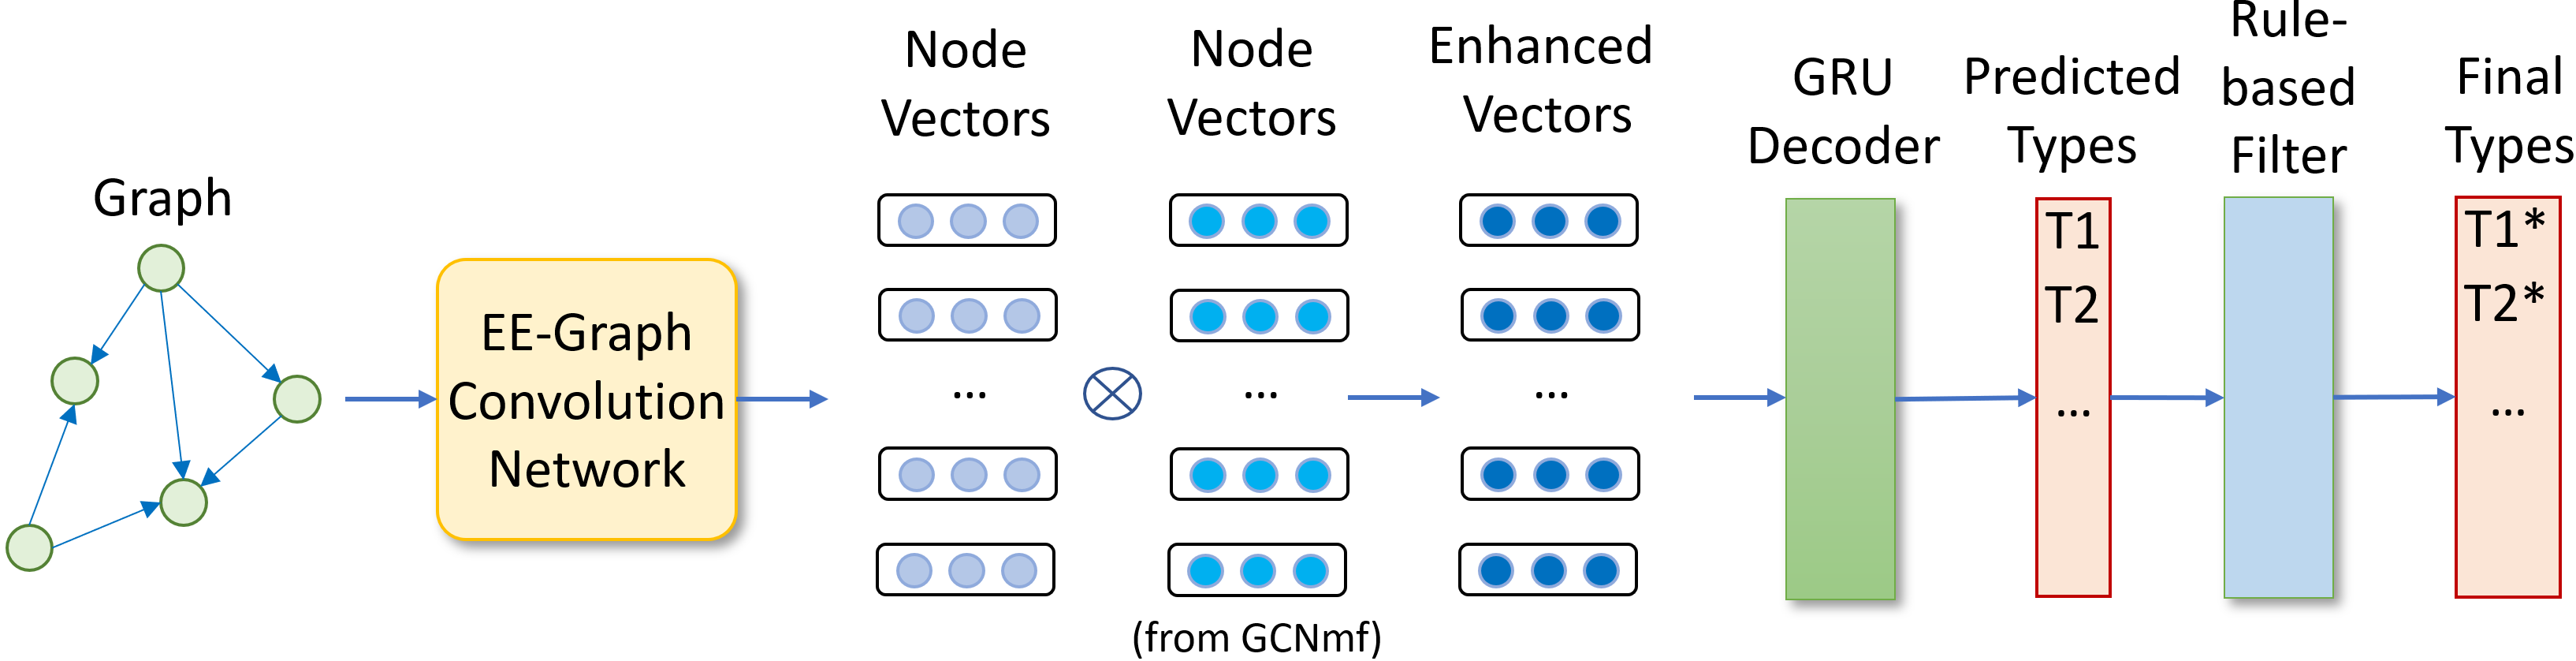
\includegraphics[width=4.8in]{figures/type-gen-model-2}
          \vspace{-6pt}
		\caption{Variable Type Generation Model (VTG)}
		\label{fig:type-gen}
	\end{center}
\end{figure*}

This section presents the Variable Type Generation Model (VTG).  The
input is the minified code with all the original variables' names and
types during training, and without the types during
prediction. Similar to VNG model, the combined graph $G$ is processed
in which the names in the code sequence of each node $n$ is tokenzed
and an embedding model is applied to build the vector for $n$
considering each sequence of sub-tokens for $n$ as a sentence.

%During training, the input is the minified code with all the original
%variables’ names and types, and during predicting, it does not have
%them. First, we build the TDG and the RG for the given minified code.
%The two graphs are combined into a representation graph $G$. For each
%node in $G$, we tokenize the names in the corresponding code sequence
%of the node. We consider each of them as a sentence and use an
%embedding model (e.g., GloVe~\cite{pennington2014glove}) to build the
%representation vector for each node in $G$.

Next, we feed the graph $G$ with those vectors to Edge-Enhanced Graph
Convolutional Network (EE-GCN)~\cite{ee-gcn}. EE-GCN could accept both
node and edge features.  We use the above vectors as node features,
and the edge types in the graph $G$ (built from TDG and RG) as
the edge features.
%
{\color{blue}{The rationale for choosing EE-GCN is its capability
    producing the embeddings emphasizing on the edges in $G$, which
    represent the relations/dependencies among the data types.
%
A key characteristic of EE-GCN is that it has an edge-aware node
update module and a node-aware edge update module, and two modules
work in a mutual way by updating each other
iteratively. Specifically, ``for each layer, the edge-aware node
update module is first performed for aggregating information from
neighbors of each node through specific edges. Then, a node-aware edge
update module is used to dynamically refine the edge representation
with its connected node representations, making the edge
representation more informative.''}}  The output of the EE-GCN model
includes the list of the representation vectors $V_n$ for all the
nodes in $G$.

To further propagate the impact from variable name learning to type
learning, we combine the above vectors $V_n$ with the vectors obtained
from the GCNmf in the Variable Name Generation model. Specifically, we
use the cross-product between the two vectors to produce the final
vectors $V_f$ for the type prediction for all the nodes. Next, we
leverage a Gate Recurrent Unit (GRU) as a decoder, which accepts the
vectors $V_f$s as input and generates the type for the node. (During
training, the type labels are used). {\color{blue}{{\tool} handles the
    primitive and non-primitive types in the same way as the decoder
    generates them as texts for the type names}}.
%
Finally, we also apply the rule-based filter, which performs
type-checking to eliminate the candidates that violate the type
inference rules.
%
{\color{blue}{In the current implementation, we used a small subset of
the static type inference rules for
    Python~\cite{type-system-python}. For example, we check the types
    of the left-hand-side and the right-hand-side of an assigment, the
    type of the condition in an \code{if} statement, the type of a
    comparison operation, the simple sub-typing rules for primitive
    types and for lists, tuples, and dictionaries, etc.}}
%
The final result include the types for all the nodes including the
ones for variables.

%6> When generating the type, we use some basic rule from parser to
%reduce the possible candidates.

%Variable Type Generation:

%1> Graph edge represent different relations (This may change depends on the graph we finally want to use). Each node is a variable, method call, or a field of an object. We use the name of the variable (minified), method call, or the field as the node feature and use GloVe to learn the representation vector.

%2> We use EGCN that accepts graphs with both node features and edges features as input. Here the edge feature is the edge type.

%3> The output of EGCN is the generated representation vector $V_r$ for each node.

%4> We combined the representation vector we get from EGCN with the generated from the next step $V'_r$ (variable name generation) by using the cross-product and get the final generated representation vector for type prediction ($V_f$)

%5> We use a GRU (RNN) as decoder accepts the $V_f$ as input and generates the type for the variables as output.

%6> When generating the type, we use some basic rule from parser to reduce the possible candidates.
